\chapter{Cyfrowy system wizyjny}
\label{cha:csw}

\section{Metody akwizycja obrazu i kalibracja}

Większość implementacji wykorzystuje układ dwóch równoległych do siebie kamer. Do połączenia obrazów należy zastosować algorytm wyrównujący oba obrazy. Kalibrację wykonuję się specjalnymi  planszami które pozwalają określić położenie punktów kalibracyjnych w obu rejestrowanych zakresach. Plansze mogą być aktywne (posiadają własne źródło ciepła) albo pasywne (przesłaniają obce źródło ciepła). W tym układzie występuję również zjawisko paralaksy które powiększa się wraz z wzrostem odległości obiektu od punktu kalibracji. W pracy  \cite{hwang2015multispectral} autorzy zastosowali zwierciadło półprzezroczyste wykonane z wafla krzemowego pokrytego cynkiem do rozdzielenia obrazu co wyeliminowało wady układu równoległego.

\begin{figure}[h]
	\centering
	\begin{subfigure}{0.45\textwidth}
		\centering
		 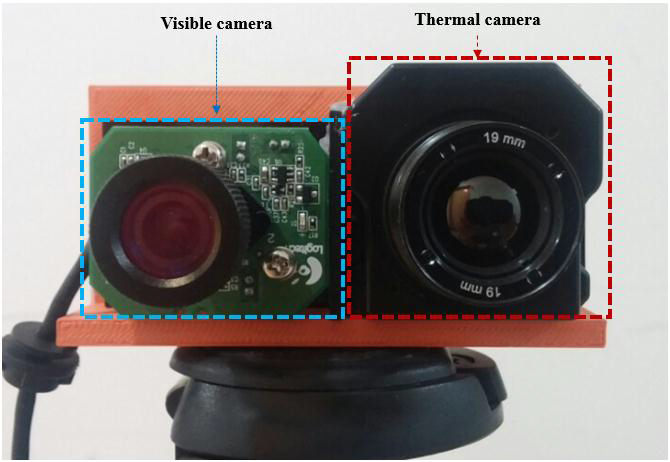
\includegraphics[width=1\textwidth]{images/dual-camera}
		\subcaption{\label{dual_camera}}
	\end{subfigure}
	\begin{subfigure}{0.45\textwidth}
		\centering
		 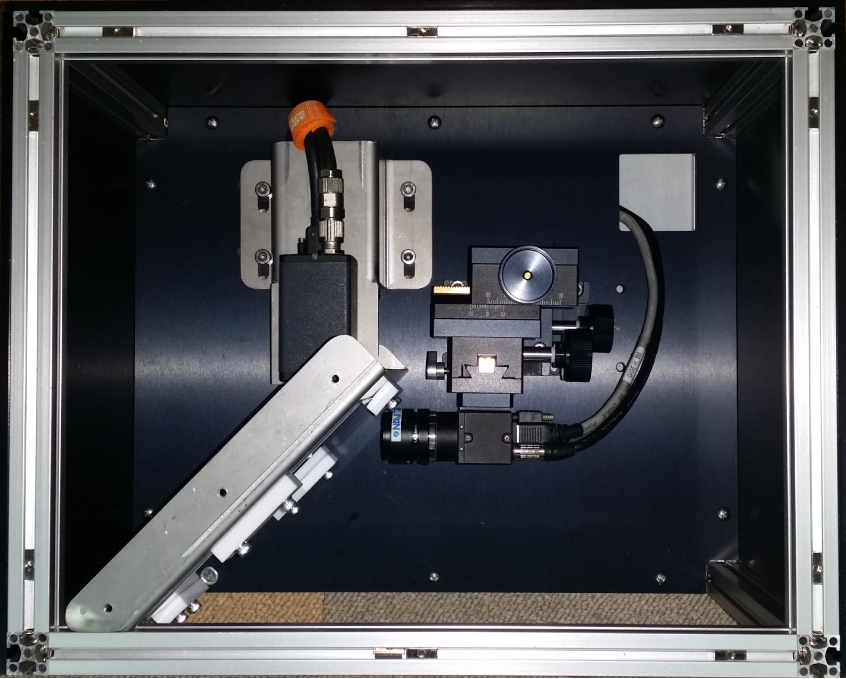
\includegraphics[width=1\textwidth]{images/multispectral}
		\subcaption{\label{multispectral}}
	\end{subfigure}
	
	\caption{\label{fig:cameras_systems}Sposoby akwizycji obrazów:  \protect\subref{dual_camera} dwie kamery równolegle \cite{lee2015robust}, \protect\subref{multispectral} z wykorzystaniem zwierciadła półprzezroczystego \cite{hwang2015multispectral}.}
\end{figure}

\section{Model geometryczny}

Do opisu matematycznego systemu wykorzystuje się model kamery otworowej. Dzięki niej można opisać relację między trójwymiarową przestrzenią a dwuwymiarowym obrazem za pomocą projekcji perspektywicznych. Nie stanowi on najdokładniejszego opisu matematycznego kamery, nie ma uwzględnionych w nim zakłóceń soczewkowych, ale jest wystarczające dobre dla niektórych zastosowań. Składa się ona z 2 zestawów parametrów: zewnętrznych oraz wewnętrznych. Parametry zewnętrzne definiują lokację kamery względem zewnętrznego układu współrzędnych. Są reprezentowane przez wektor translacji \(T\) między układem związanym z kamerą \( \left (  X_{c},Y_{c},Z_{c}\right ) \)
 a zewnętrznym \(\left (  X,Y,Z\right )\). Drugim parametrem jest macierz rotacji \( R \)( między osiami tych dwóch układów.
Punkt \(P = \left [ X,Y,Z \right ]^T \) będący w zewnętrznym układzie współrzędnym ma swój odpowiednik w układzie wewnętrznym który można określić zależnością 

\begin{equation}
P_{c} = RP+T
\end{equation}

Właściwości optyczne kamery można przedstawić w postaci macierzy kamery.

\begin{equation}
K = \begin{bmatrix}
f_x & 0 & x_0 \\ 
0 & f_y & y_0\\ 
0 &0  & 1
\end{bmatrix}
\end{equation}
gdzie:
\begin{conditions}
f_{x}, f_{y} & ogniskowa kamery wyrażona w liczbie pikseli, \\
x_{0},y_{0} & współrzęne punktu głównego. 
\end{conditions}

Macierz K określa związek między między znormalizowanymi współrzędnymi w układzie odniesienia kamery, danych wzorem \(x_n = \frac{X_c}{Z_c}, y_n = \frac{Y_c}{Z_c}\), a odpowiadającym im wspórzędnymi punktów na obrazie \(u,v\):

\begin{equation}
\begin{bmatrix}
u \\
v \\
1
\end{bmatrix} = K \begin{bmatrix}
x_n \\
y_n \\
1
\end{bmatrix}
\end{equation}
W pracy \cite{rangel20143d} autorzy sprawdzili kila różnych plansz kalibracyjnych i najlepsza okazała się z kartonu... TO DO: dopisać.


\section{Algorytmy detekcji pieszych}

W cyfrowej analizie obrazu rozpoznawanie pieszych jest jedną z najbardziej aktywnych i rozwijanych dziedzin. W przeciągu kilkudziesięciu lat powstało ponad tysiąc artykułów poruszających to zagadnienie \cite{zhang2015filtered} i wiele różnych metod zostało już opracowanych. Większość metod opiera się o analizę obrazu tylko w jednym spektrum: widzialnym albo podczerwieni. Praca \cite{hwang2015multispectral} pokazała że połączenie obu obrazów może dać lepsze wyniki. Podobnie w \cite{gonzalez2016pedestrian} ustalono że analiza multispektralna jest skuteczniejsza w dzień niż w nocy (o około 5\% AMR (ang. avrange miss rate).   W artykule \cite{benenson2014ten} autorzy podsumowują osiągnięcia w dziedzinie detekcji pieszych w latach 2004 – 2014 wyróżniono ponad 40 różnych podejść do problemu. Artykuł jest oparty o bazę danych Caltech-USA która oferuje obrazy w kolorze. Jednym z wniosków jest że przez ostanie dziesięć lat największy postęp został osiągnięty głównie dzięki dopracowaniu cech jakie są wyodrębniane z obrazu niż ulepszanie klasyfikatora. Dodatkowo autorzy połączyli cechy dające najlepsze wyniki i stworzyli własną metodę która uzyska 12\% zysk AMR względem  najlepszej badanej wcześniej metody.

Dla typowego algorytmu detekcji pieszych można wyróżnić trzy podstawowe etapy:

\subsection{Ustalenie regionu zainteresowań} 
Jest to obszar zwany ROI(ang. Region of interest) w którym potencjalnie mogą znajdować się przechodnie. Wiele podejść uznaje cały obraz jako ROI i stosuje okno przesuwne sprawdzając każdy możliwy fragment obrazu. Jeżeli obraz jest rejestrowany przez nieruchomą kamerę, ROI można określić poprzez różnicę między zapamiętanym tłem a aktualnym obrazem. Wyodrębnienie ROI jest bardzo istotne w przypadku pracy w czasie rzeczywistym ze względu na ograniczony czas analizy pojedynczego obrazu.

\subsection{Wyodrębnienie cech}
Do najbardziej popularnych cech można zaliczyć:

\begin{enumerate}
\item Histogramy zorientowanych gradientów (HOG) zaproponowany przez N.Dalala i B. Triggs w pracy \cite{dalal2005histograms} stała się jedną z najbardziej popularnych techniką w dziedzinie rozpoznawania ludzi. Jest cały czas rozwijana i modyfikowana w wielu pracach naukowych. Technika polega na zliczeniu kierunków gradientów, uzyskanych z 2 masek kierunkowych \(\begin{bmatrix}-1 & 0 & 1\end{bmatrix} \) i \( \begin{bmatrix}-1 & 0 & 1 \end{bmatrix}^T\), w komórkach o określonych wymiarach. Komórki te są organizowane w bloki w obrębie których następuję normalizacja. Wektorem cech jest połączony wszystkich histogramów z wszystkich bloków w jeden wektor.

\item Lokalne wzorce binarne LBP (ang. Local Binary Paterns). 

\item Falki Haara.

\item Kolor. W analizie obrazo wykorzystuje różne przestrzenie barw np. RGB, HSV oraz LUV

\item Lokalna struktura. W odróżnieniu od pojedynczych pikseli można wyznaczyć lokalne struktury o podobnym kolorze. (np. głowa i ręce mają podobne kolory, jednolita koszula, spodnie)

\item i wiele innych

\end{enumerate}

\subsection{Klasyfikator}
Otrzymany wektor cech jest poddany klasyfikacji której wynik decyduje czy obraz zawiera człowieka. W pracy \cite{benenson2014ten} autorzy wyróżnili 3 dominujące rodziny:

\begin{enumerate}
\item Rodzina DPM (ang. Deformable Part Detectors) ??? wykrywacze deformowlnych elementów ???. Technika polega na klasyfikacji poszczególnych elementów człowieka (głowa, tułów, nogi). Następnie  jest analizowany układ tych elementów na obrazie i podjęcie decyzji o obecności człowieka.

\item Deep networks – głębokie sieci neuronowe.

\item Decision forests – ?? lasy decyzyjne ?? zbiór nieskorelowanych drzew decyzyjnych.

\item inne: SVN (ang. support vector machine – maszyna wektorów nośnych), AdaBoost itp.
\end{enumerate}

\section{Wykorzystanie FPGA w analizie obrazu}

	Tradycyjne systemy wizyjne zwykle bazują na architekturze sekwencyjnej, po kolejnym przekształceniu obraz jest sukcesywnie poddawany następnym. W aplikacji procesorowej te operacje są wykonywane przez układ arytmetyczno-logiczny w który jest wyposażony. Kolejne kroki algorytmu są kompilowane w ciąg instrukcji dla procesora który oprócz operacji matematycznych dużą część pracy poświęca na pobieranie i dekodowanie rozkazów oraz na pobieranie i zapisywanie danych do pamięci. By taka aplikacja mogła pracować w czasie rzeczywistym cała procedura musi wykonać się szybciej przychodzące dane obrazu co wymusza wysoki taktowanie procesora sięgające GHz. 
	W przypadku podejścia równoległego, implementacja poszczególnych kroków algorytmu odbywa się w osobnych procesach. Jeżeli kolejne kroki algorytmu wymagałyby danych otrzymanych z poprzednich to zysk takiego zabiegu byłby równy zero.  By uzyskać znacznie przyspieszenie algorytm musi mieć możliwość podzielenia na wiele niezależnych części. Maksymalne do uzyskania przyspieszenie jest określone przez prawo Amdahla: 
\begin{equation}
P_w =\frac{1}{ s + \frac{1-s}{n_w}}
\end{equation}
gdzie:
\begin{conditions}
P_{w} &  przyspieszenie algorytmu w systemie wieloprocesorowym, \\
s &  cześć algorytmu niepodlegająca zrównolegleniu (wartość od zera do jeden), \\
n_{w} & liczba elementów obliczeniowych.
\end{conditions}

Teoretycznie jedynym ograniczaniem w możliwości zrównolegnia obliczeń jest ilość zasobów dostępnych, jednak istotnym aspektem jest sposób dostarczania danych do zaimplementowanych w układzie procesorów. Czas i przepustowość jaka jest potrzebna do odczytania i zapisu obrazu po przetworzeniu z i do pamięci jest najczęściej wąskim gardłem systemu wizyjnego. Z tego powodu przetwarzanie obrazu bezpośrednio z sensora w czasie jego akwizycji jest chętnie wykorzystywane gdyż zmniejsza to ilość operacji odczytu i zapisu.  \cite{garcia2014survey}

\section{Podejście sprzętowo - programowe}

W pracy \cite{honegger2014real} autorzy wykorzystali układ FPGA oraz CPU małej mocy do skonstruowania systemu wizyjnego dla robotów. System analizował obraz steroskopowy z dwóch kamer tworząc mapę głębi. Obie kamery są bezpośrednio podpięte do układu FPGA w którym obrazy są przetwarzane. Następnie dwa oryginalne obrazy oraz mapa głębi są przesyłane do CPU za pomocą specjalnej szyny danych. Moduł frame grabbera przechwytywał ten obraz i wykorzystując DMA (ang. Direct Memeory Acces) zapisywał do pamięci systemu. Ten zabieg gwarantował poprawną transmisję obrazu do CPU. Rozdzielczość oraz ilość klatek na sekundę są w pełni elastyczne dzięki czemu CPU dostawało obraz o szerokości trzy raz większej niż oryginalny obraz. Pozwalało to na przesłanie zsynchronizowanego lewego, prawego obrazu i mapy głębi. System pracował w rozdzielczości 752x480 piksle i 60 klatkach na sekundę. Całość systemu wizyjne włącznie z kamerami, układem FPGA, CPU oraz konwerterami napięcia pobierał mniej niż 5W mocy. Całkowita latencja podana przez autorów rozwiązania wynosi około 2ms.

W pracy \cite{piao2016real} autorzy wykorzystali układ SoC (ang. System on Chip) do detekcji pieszych dla zaawansowanego systemu wspomagania kierowcy (ADSA ang. advanced driver assistance system). Głównym wyzwaniem było opracowanie metody która działa w czasie rzeczywistym, ma mały pobór mocy oraz niski koszt wykonania. Większość topowych algorytmów  wymaga znacznych zasobów obliczeniowych więc autorzy dokonali relaksacji problemu poprzez zastosowanie prostszego deskryptora jakim jest LBP oraz SVM jako klasyfikatora. Autorzy zamontowali po każdej stronie pojazdu inteligentną kamerę o 180$^\circ$ horyzontalnym kącie widzenia by jak najlepiej monitorować przestrzeń wokół niego. W kamerach została przeprowadzona wstępna obróbka obrazu (rektyfikacja i skalowanie). Przetworzony obraz z kamer był transmitowany do „Fusion-Box” gdzie odbywała się generacja kandydatów, klasyfikacja, weryfikacja oraz śledzenie. Wyniki były przesyłane do wbudowanego komputera PC. Rozwiązanie nie zostało jeszcze w pełni zaimplementowane ale pierwsze testy dawały obiecujące rezultaty.

\section{Sprzęt}
\subsection{Kamera termowizyjna Lepton} 
Lepton jest zintegrowaną w pojedynczym układzie kamerą składającą się z soczewki, sensora podczerwieni fal długich (ang. LWIR – long wave infrared) oraz elektroniki sterującej i przetwarzającej sygnał.  Układ ma możliwość domontowania dodatkowej przesłony która jest wykorzystywana do automatycznej optymalizacji procesu ujednolicania obrazu (kalibracji sensora).
Prosty do integracji z dowolnym mikrokontrolerem dzięki zastosowaniu standardowych protokołów i interfejsów. Lepton po podłączeniu od razu pracuję w domyślnym trybie pracy, który może zostać zmieniony za pomocą CCI (ang. camera control interface – interfejs kontroli kamery).\cite{lepton}
Parametry:
\begin{itemize}
\item Wymiary: 11,8 x 12,7 x 7,2 mm, 
\item Sensor: niechłodzony mikrobolometr VOx (tlenek wanadu),
\item Rejestrowany zakres: fale długie podczerwieni, 8$\mu$ m do 14$\mu$ m ,
\item Wielkość piksela: 17 $\mu$m,
\item Rozdzielczosć: 80x60 pikseli,
\item Ilość klatek na sekundę 8,6,
\item Zakres rejestrowanych temperatur: -10  $^\circ$  C 140  $^\circ$  C (Tryb wysokiego wzmocnienie),
\item korekta niejednorodności matrycy: automatyczna na bazie przepływu optycznego
\item kąt widzenia horyzontalny / diagonalny: 51 $^\circ$ \\ 66 $^\circ$,
\item Głębia ostrości: od 10cm do nieskończoności
\item Format wyjściowy: do wyboru: 14-bit, 8-bit (z AGC (ang. automatic gain control – automatyczna kontrola wzocnienia)) 24-bit rgb (z ACG i koloryzacją).
\item Interfejs video: VoSPI (Video over Serial Peripherial Interface)
\item Interfejs sterujący: CCI (I2C podobny)
\end{itemize}
\subsection{Zynq-7000}

Rodzina układów Zynq-7000 bazuje na architekturze SoC (ang. System on Chip). Posiadają zintegrowany kompletny system składający podzielonego na dwie części: systemu procesorowego bazującego na procesorze ARM Cortex-A9 (PS ang. Porcessing System) oraz logikę programowalną (PL ang. programable logic) FPGA w jednym układzie scalonym. Na rysunku \ref{fig:zynq7000} przedstawiono schemat architektury. Prócz procesora cześć procesorowa posiada wbudowaną pamięć, kontroler pamięci zewnętrzne oraz szereg interfejsów dla układów peryferyjnych takich jak USB, GigEthernet, CAN, I2C, SPI. W części logiki programowalnej znajdują się bloki logiki konfigurowalnej (CLB ang. configurable logic block), 36Kb bloki pamięci RAM, procesory sygnałowe DSP48, układ JTAG, układy zarządzania zegarami oraz dwa 12-bitowe przetwornik analogowo-cyfrowy.

Komunikacji między częścią procesorową a logiką programowalną odbywa się za pośrednictwem Interfejsu AXI (ang. Advanced Extensible Interface), oraz bezpośrednio wykorzystując porty generalnego przeznaczenia, przerwania, oraz poprzez bezpośredni dostęp do pamięci (DMA ang. Direct Memory Access) 

\begin{figure}[h]
    \centering
    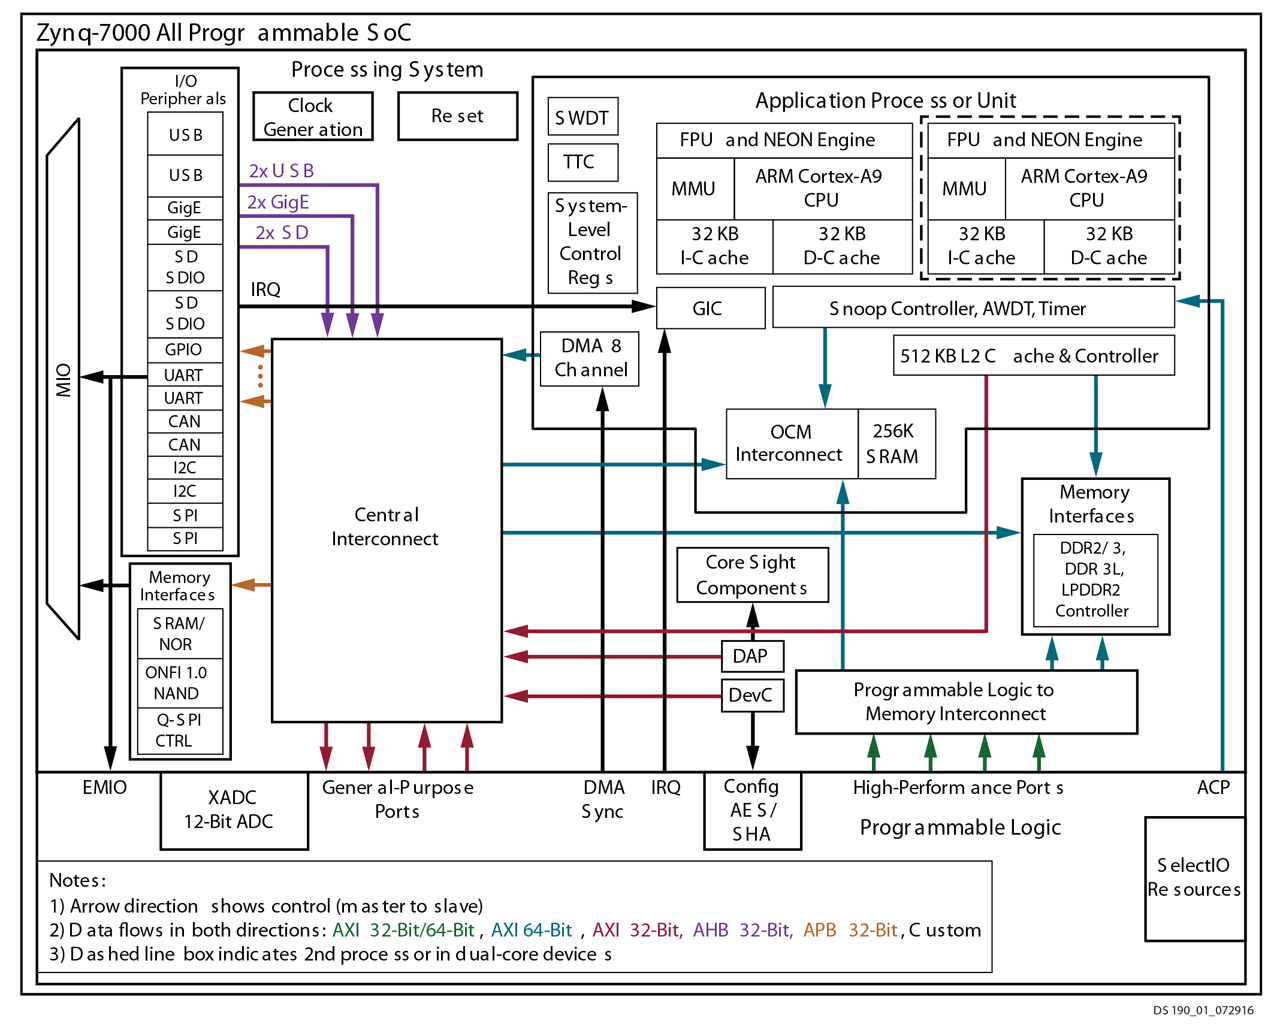
\includegraphics[width=1\textwidth]{images/Zynq-7000-Overview}
    \caption{Schemat ogólny architektury układu Zynq-7000.}
    \label{fig:zynq7000}
\end{figure}

\section{Interfejs AXI}
 AXI (ang. Advanced eXtensible Interface zawansowany rozszerzalny interfejs) jest częścią ARM AMBA (ang. Advanced Microcontroller Bus Architecture) – otwartego standardu, specyfikacją do zarządzania i połączeń między blokami funkcyjnymi w SoC. Aktualnie jest stosowana AMBA 4.0 która wprowadziła drugą wersję AXI, AXI4. Występują trzy typy interfejsów dla AXI4:
\begin{itemize}
\item AXI4 – stosowany w wysokowydajnych transferach w przestrzeni pamięci (ang. memory-mapped)
\item AXI4-Ligt – stosowany dla prostszych operacji w przestrzeni pamięci (na przykład do komunikacji z rejestrami kontrolnymi i statusu)
\item AXI4-Stream – stosowany do wysokiej prędkości transmisji strumieniowych
\end{itemize}
Specyfikacja interfejsu zakłada komunikację pomiędzy pojedynczym AXI master i pojedynczym AXI slave, która ma na celu wymianę informacji pomiędzy tymi dwoma blokami funkcyjnymi IP core. Kilkanaście interfejsów AXI master i slave mogą zostać połączone między sobą za pomocą specjalnej struktury zwanej interconnect block (blok międzypołączeniowy) w której odbywa się trasowanie połączeń do poszczególnych bloków. 

AXI4 i AXI4-Lite składają się z 5 różnych kanałów:
\begin{itemize}
\item Kanał adresu odczytu,
\item Kanał adresu zapisu,
\item Kanał danych odczytanych
\item Kanał danych do zapisania
\item Kanał potwierdzenia zapisu
\end{itemize}
Dane mogą płynąć w obie strony pomiędzy master a slave jednocześnie. Ilość danych które można przesłać w jednej transakcji w przypadku AXI4 wynosi 256 transferów, zaś AXI4-Lite pozwala na tylko 1 transmisję.

AXI4-Stream nie posiada pola adresowego, a dane mogą być przesyłane nieprzerwanie. 
\subsection{Wykorzystanie AXI-Stream do transmisji sygnału video.} 
W odróżnieniu od klasycznej implementacji przetwarzania strumieniowego video, w AXI-Stream przesyłane są jedynie aktywne piksele. Linie synchronizacji poziomej i pionowej są odrzucane albo są połączane do specjalnego bloku detekcji timingów który mierzy parametry wchodzącego strumienia wizyjnego (ilość pikseli na linie, czas ilość aktywnych linii, czas wyciemnienia itd.). Podobnie informacje o synchronizacji są dodawane przez blok generujący timingi.

Do transmisji wykorzystane jest 6 linii: jedna linia danych i pięć kontrolno-sterujących. 
\begin{itemize}
\item Video Data – linia danych o szerokości jednego (albo dwóch) pikseli. Szerokość tej linii powinna być wielokrotnością liczby osim (16, 24, 48 itd.)
\item Valid – Linia podająca czy dane piksela są poprawne,
\item Ready – Linia kontrolna informująca urządzenie master że slave jest gotowy do transmisji danych,
\item Start Of Frame – linia która wskazuje pierwszy piksel nowej ramki,
\item End Of Line – linia wskazująca ostatni piksel w linii.
\end{itemize}
Aby mógł wystąpić poprawny transfer danych linie Valid i Ready muszą być w stanie wysokim podczas rosnącego zbocza zegara. Przykładowe nawiązanie transmisji przedstawia rysunek \ref{fig:handshake}

\begin{figure}[h]
    \centering
    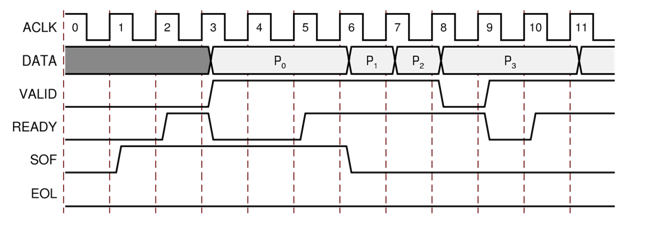
\includegraphics[width=1\textwidth]{images/axi-stream_hendshake}
    \caption{Przykład rozpoczęcia transmisji Reday/Valid.}
    \label{fig:handshake}
\end{figure}